\section{Background}
The beta exponent ($\beta$) dictates the transport capacity ($q_{s\_{}cap}$) of individual sand parcels as
\begin{equation}
	q_{s\_{}cap} = q_{s0} \frac{u_{loc}^{\beta}}{u_{0}^{\beta}},
\end{equation}
where $q_{s0}$ is the upstream sand flux input divided by the inlet channel width.
This scaling is based on the Meyer-Peter and Muller \citep{meyer1948formulas} formulation and is a nonlinear function of local flow velocity.
Therefore, by changing the value of $\beta$, the transport behavior for sand parcels can be altered for the given simulation.

\section{Model Runs}
To test the influence of the $\beta$ YAML parameter, runs with the following parameters were conducted in triplicate with beta values of $\beta = 1, 2, 3, 4, 5, 10, 15$.
The YAML below provides information about the parameter set used.\\

\noindent \texttt{YAML} configuration file: \vspace{-6pt}
\begin{boxedverbatim}
Length: 7500
Width: 15000
timesteps: 5000
L0_meters: 150.0
N0_meters: 250.0
dx: 50.0
h0: 5.0
Np_water: 2000
Np_sed: 2000
save_dt: 250000
\end{boxedverbatim}

\section{Results}
The influence of the beta parameter can be seen when looking at the final topographies generated by the various models (Figure \ref{fig:beta_topos}).

\begin{sidewaysfigure}[!ht]
	\makebox[\textwidth][c]{
	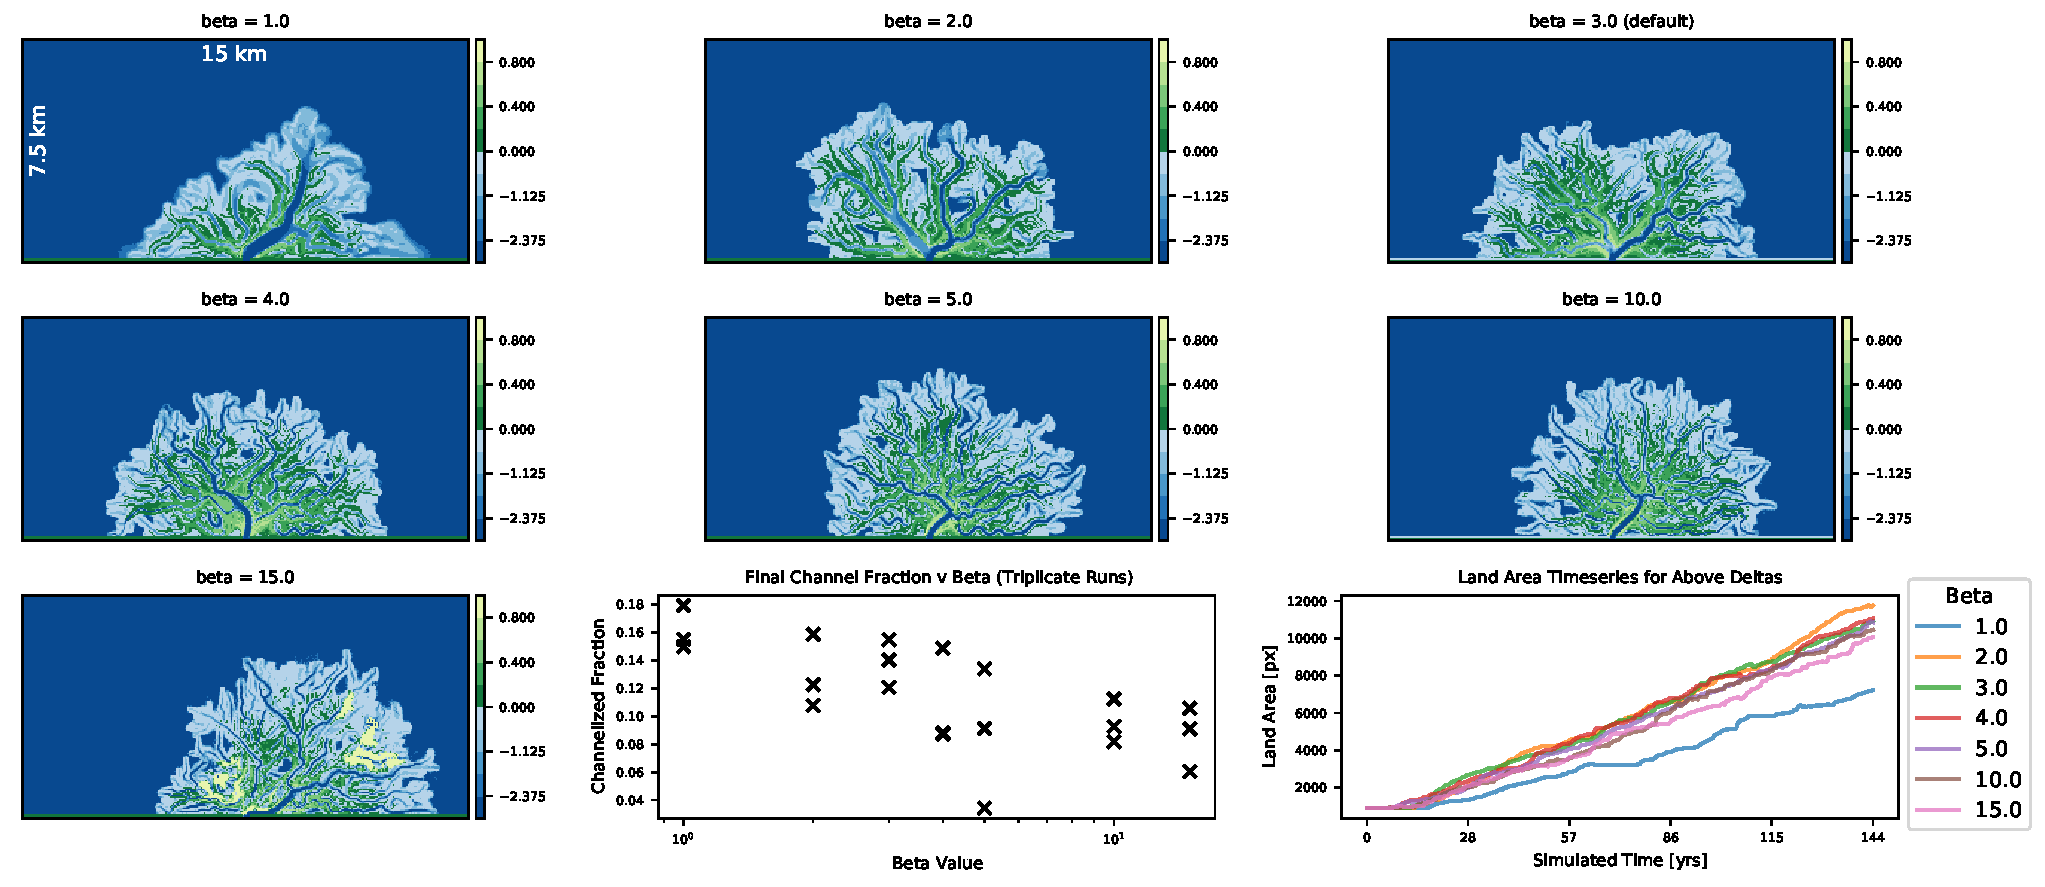
\includegraphics[width=\textwidth]{BetaImpact/figs/beta_results.pdf}
	}	
	\caption{Examples of the final topographies obtained for different values of $\beta$. \textit{Bottom, center:} Channelized fractions at the end of each model run as a function of the beta parameter. \textit{Bottom, right:} Land area timeseries for one model per beta parameter.}
	\label{fig:beta_topos}
\end{sidewaysfigure}

\begin{sidewaysfigure}[!ht]
	\makebox[\textwidth][c]{
	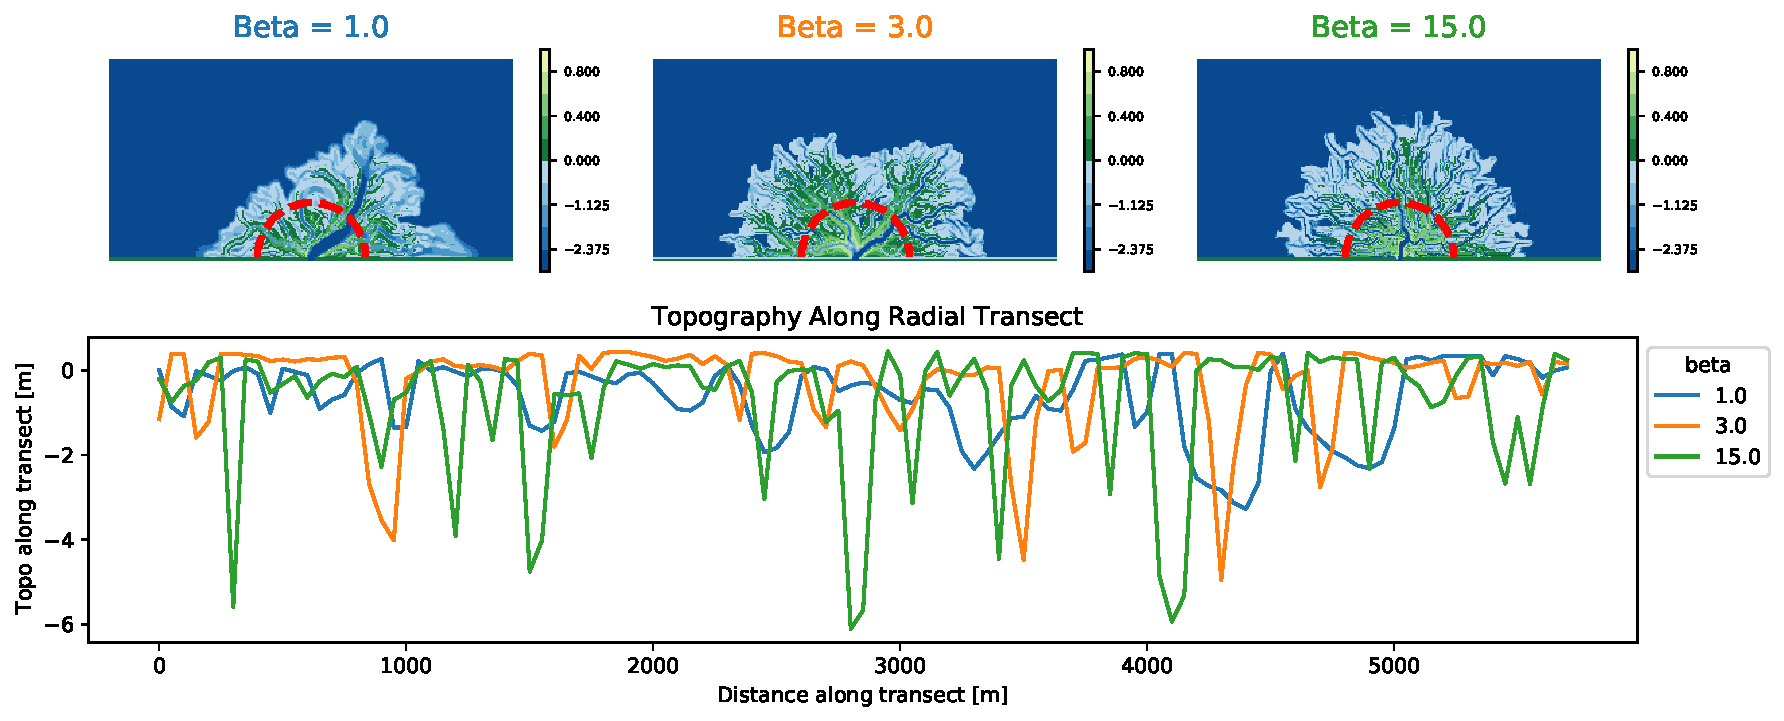
\includegraphics[width=\textwidth]{BetaImpact/figs/topotransect_beta.pdf}
	}	
	\caption{Topography transects for the lowest, default, and highest beta values tested to visualize the impact of topographic diffusion on the channel geometries.}
	\label{fig:beta_transect}
\end{sidewaysfigure}

\begin{figure}[!ht]
	\makebox[\textwidth][c]{
	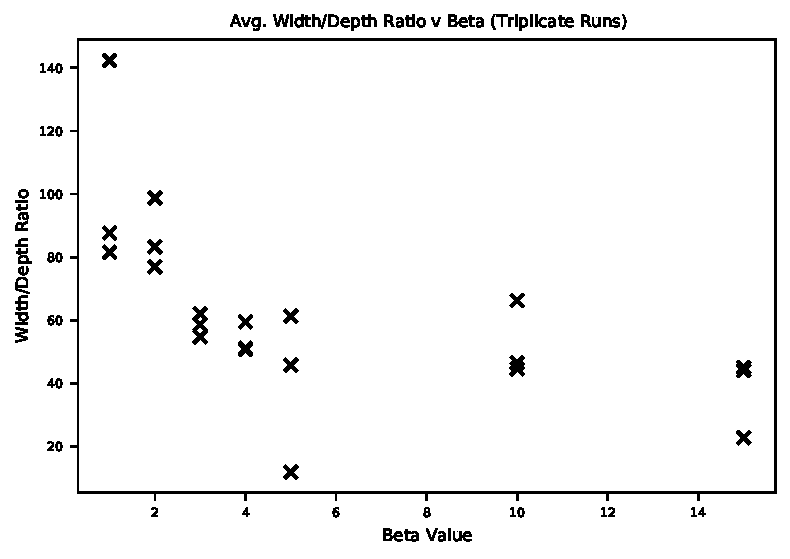
\includegraphics[width=\textwidth]{BetaImpact/figs/widthdepth_beta.pdf}
	}	
	\caption{Plot of average width-to-depth ratios as a function of the different beta values. Width-to-depth ratios are calculated along the azimuthal transects visualized in Figure \ref{fig:beta_transect}.}
	\label{fig:beta_wd}
\end{figure}

\section{Conclusions}
The beta parameter clearly influences the simulated deltas.
When $\beta$ greatly exceeds the default value of 3.0, then the model can become unstable.
Results here for $\beta$ values of 15 resulted in portions of the delta having unrealistically high elevations on the order of 1,000 meters above sea level.
Similarly when the value of beta becomes too small, the result can be unrealistic.
This is evident in the runs conducted with beta values of 1.0 in which the capacity of the sand parcels must be near-zero, and therefore the system is far to diffusive.

\clearpage
\bibliographystyle{plainnat}
\bibliography{bib/bib}